% !Mode:: "TeX:UTF-8"

%要运行该模板,LaTex需要安装CJK库以支持汉字.
%字体大小为12像素,文档类型为article
%如果你要写论文,就用report代替article
%所有LaTex文档开头必须使用这句话
\documentclass[12pt,twocolumn]{article}

%使用支持汉字的CJK包
\usepackage{CJKutf8}
\usepackage{indentfirst}
\usepackage[top=0.5in, bottom=0.5in, left=0.4in, right=0.4in]{geometry}
\usepackage[square,comma,numbers,sort&compress]{natbib}
\usepackage{graphicx}
\usepackage{booktabs}
\usepackage{tabularx}
\usepackage{enumitem}
\usepackage{titling}

\setlength{\parindent}{2em}
\setlength{\parskip}{0.5em}

\renewcommand{\contentsname}{目录}
\renewcommand{\listfigurename}{插图目录}
\renewcommand{\listtablename}{表格目录}
\renewcommand{\refname}{参考文献}
\renewcommand{\abstractname}{摘要}
\renewcommand{\indexname}{索引}
\renewcommand{\tablename}{表}
\renewcommand{\figurename}{图}

\setlength{\abovecaptionskip}{0em plus 0.3em minus 0.3em}
\setlength{\belowcaptionskip}{0em plus 0.3em minus 0.3em}
\setlength{\tabcolsep}{0.5em}
\setlength{\columnsep}{0.4in}

\linespread{1.1}

\setlist[1]{itemsep=0em,topsep=0em}

\renewcommand{\arraystretch}{1.3}

% make title left
\makeatletter
\renewcommand{\maketitle}{\bgroup\setlength{\parindent}{0pt}
\begin{flushleft}
  \LARGE {\textbf{\@title}}\vspace{1em}

  \normalsize{\@author}
\end{flushleft}\egroup
}
\makeatother

% change margin
\def\changemargin#1#2{\list{}{\rightmargin#2\leftmargin#1}\item[]}
\let\endchangemargin=\endlist

%开始CJK环境,只有在这句话之后,你才能使用汉字
%另外,如果在Linux下,请将文件的编码格式设置成GBK
%否则会显示乱码
\begin{CJK*}{UTF8}{gbsn}
\CJKindent
\CJKtilde

%这是文章的标题
%\title{动态图的可视分析方法综述}

%这是文章的作者
%\author{王祖超\hspace{1em}袁晓如}

%这是文章的时间
%如果没有这行将显示当前时间
%如果不想显示时间则使用 \date{}
\date{}

%以上部分叫做"导言区",下面才开始写正文
\begin{document}

\twocolumn[
  \begin{@twocolumnfalse}
    %这是文章的标题
    \title{动态图的可视分析方法综述}
    %这是文章的作者
    \author{王祖超\hspace{1em}袁晓如}
    %先插入标题
    \maketitle
    %\vspace{-4em}

    \begin{changemargin}{0.2in}{0in}
    {\bf 摘\hspace{1em}要:}轨迹数据大量产生于交通、气象、生态和移动服务等领域。
    有效的理解和利用这些数据不仅需要自动高效的分析方法,也需要直观生动的可视化。
    这两者相互结合形成了可视分析技术。本文概述了轨迹数据可视分析中的主要方法和交互技术,
    并对相关文献进行综述。最后本文总结了轨迹数据可视分析研究中的问题和挑战。
    \vspace{1em}

    {\bf 关键词:}可视分析,轨迹数据,交通数据,移动数据
    \vspace{1em}
    \end{changemargin}

    %这是文章的标题
    \title{Visual Analysis of Trajectory Data}
    %这是文章的作者
    \author{Zuchao Wang\hspace{1em}Xiaoru Yuan}
    %先插入标题
    \maketitle
    %\vspace{-4em}

    \begin{changemargin}{0.2in}{0in}
    {\bf Abstract: } Large volumes of trajectory data are generated in transportation, meteorology, ecology and location based services. Effective understanding and utilization of such data require not only efficient automatic analysis, but also intuitive and vivid visualization. Visual analysis is the combination of analysis and visualization. In this paper, we will introduce the major methodologies and interaction techniques in trajectory visual analysis. We will also summarize the problems and challenges in this research area.
    \vspace{1em}

    {\bf Keywords: }Visual Analysis, Trajectory Data, Transportation Data, Movement Data
    \vspace{2em}
    \end{changemargin}
  \end{@twocolumnfalse}
]

%再插入目录
%\tableofcontents
%\section{引言}
%\label{section:introduction}




可视分析结合了可视化、人机交互和自动分析,并使数据分析过程透明化。在一个典型的可视分析流程中~\citep{KeimAFGKM2008}~,
自动分析的结果通过可视化展示给用户,用户通过人机交互技术评价、修改和改进自动分析模型,从而得到新的自动分析结果。
这其中,由人来定义分析任务和识别复杂的模式,由机器来存储和分析大量的数据。分析结果的可视化则成为人与机器合作的桥梁。
可视分析技术使得人们可以从轨迹数据中得到更多更有用的知识。

在进行可视分析前,轨迹数据一般需要经过一些预处理,包括轨迹的切分重建、清理、压缩和存储。
特别的,对于车辆轨迹数据来说,一般还需要进行路网绑定处理将轨迹的采样点对应到道路上。
这些预处理工作一般都通过自动算法完成~\citep{WangLYZW2013,ParentSRAAB2013,ZhengZ2011}~。

在可视分析中,人们关注的研究对象一般包括移动物体、空间区域、
时间特征和移动事件~\citep{AndrienkoABKW2013}~。分析中会涉及各式各样的轨迹参数~\citep{DodgeWL2008}~,
既包括最原始的位置、时间参数,也包括派生得到的距离、方向、空间分布、加速度等参数。基于这些参数可以定义出一系列移动特征,
可以分为一般特征和行为特征。其中一般特征适用于所有轨迹,但缺少语义信息;而行为特征通常对应了移动物体的具体行为,
有很强的语义性。在不同的应用场景中可以定义不同的行为特征。

在过去几十年间,国内外的研究者们在轨迹数据可视分析方面做了大量的研究工作,其中涉及的可视分析方法多种多样。
如图~\ref{fig:overview_method}~所示,根据在分析流程中位置的不同,
这些方法大体可以分为以下三类~\citep{AndrienkoADFW2008}~:

\begin{itemize}
	\item {\bf 直接可视化:}一一将每条轨迹绘制出来。
	\item {\bf 聚集可视化:}先计算轨迹的聚集数据,然后再绘制这些聚集数据。
	\item {\bf 特征可视化:}先计算出轨迹的特征,然后通过直接或者聚集的方法绘制这些特征。
\end{itemize}

\begin{figure*}[!htb]
\centering
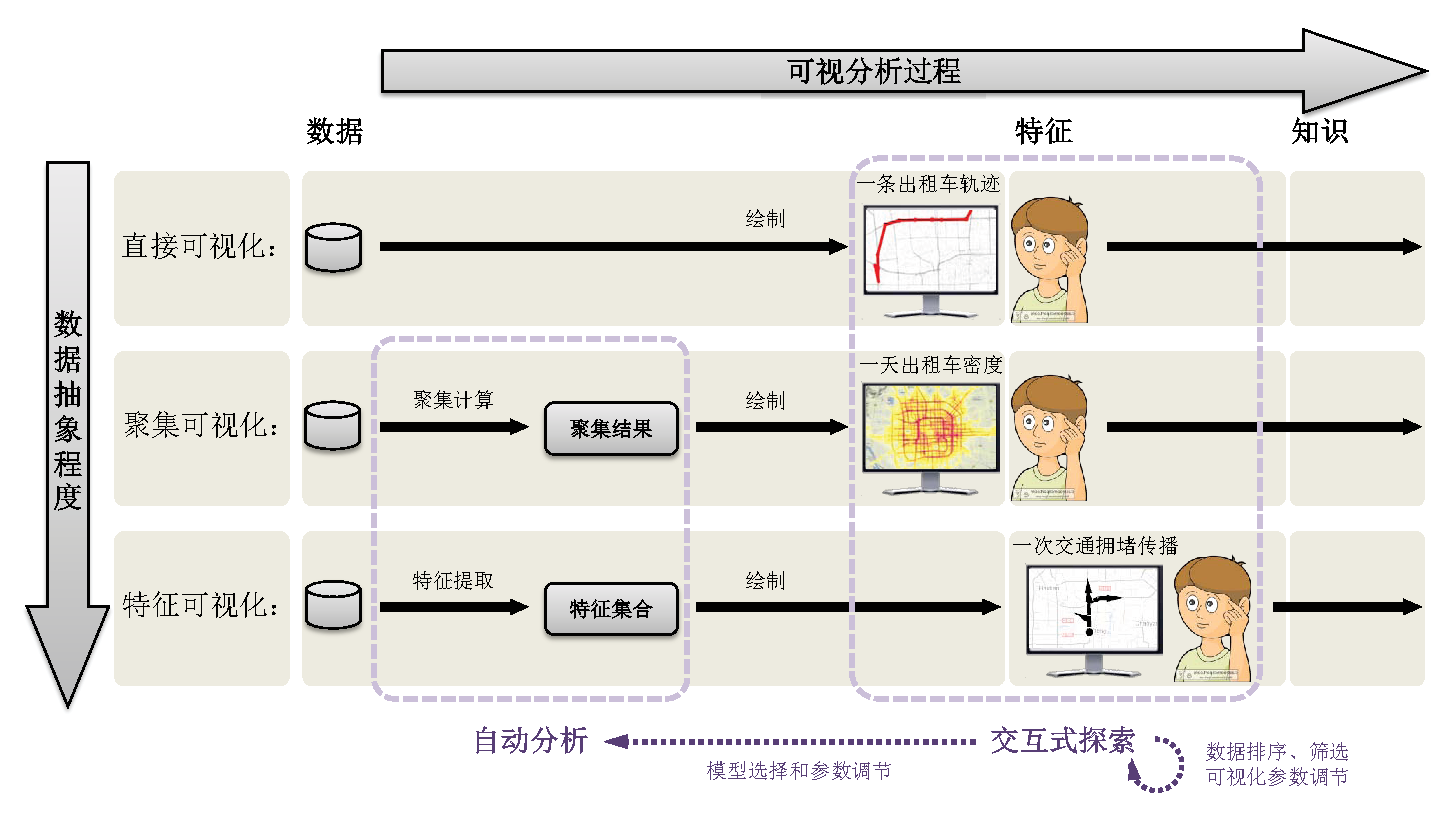
\includegraphics[width=0.85\linewidth]{images/methodoverview.eps}
\caption{\label{fig:overview_method}轨迹数据可视分析的三种方法。本图修改自Andrienko~等人的论文~\citep{AndrienkoADFW2008}~。
%轨迹数据可视分析的三种方法:直接可视化、聚集可视化和特征可视化。
%本图修改自Andrienko~等人的论文~\citep{AndrienkoADFW2008}~,其中的可视化例子来自Wang~等人的论文~\citep{WangLYZW2013}~。
}
\end{figure*}

近年来,~Andrienko~等人相继发表了轨迹数据可视分析的英文综述论文~\citep{AndrienkoA2013}~和
英文著作~\citep{AndrienkoABKW2013}~。本文将在其基础上进行进一步总结,以中文进行介绍。
相较于~Pu~等人前几年发表~\citep{PuQN2012}~的中文综述论文,本文加入了近年来的许多新工作,
并将更详尽的介绍各类可视分析方法,总结目前研究的问题和挑战。
本文将更多关注可视化的部分。关于自动分析的部分可以参考~Zheng~等人~的著作~\citep{ZhengZ2011}~。

本文将依次在第~\ref{section:direct}~、~\ref{section:aggregration}~、~\ref{section:extraction}~节介绍三种可视分析方法,
接着在第~\ref{section:interaction}~节介绍交互方法。最后,本文将在第~\ref{section:challenge}~节介绍轨迹数据可视分析的问题与挑战,
并第~\ref{section:conclusion}~节进行总结。

\section{直接可视化}
\label{section:direct}

直接可视化是最基本的可视分析方法。轨迹被一一绘制出来,显示给用户观察。在这种方法中,
计算机做的主要是“可视”的部分,而“分析”大部分依靠人来完成。

直接可视化的优点包括:

\begin{itemize}
	\item 几乎不对数据做任何假设和建模,因此可以较好的容忍数据中的噪音和异常值。
	\item 不要求有明确的分析任务,因此很适合进行探索式分析。
	\item 不需要进行特别的计算,结果简单明了,而且最准确的保留了数据中的信息。
	\item 方法简单直接,易于编程实现。
\end{itemize}

然而,由于直接可视化方法过于直接,它也有以下缺点:

\begin{itemize}
	\item 不适用于大量轨迹的分析,当轨迹很多时,相互间的遮挡将非常严重。
	\item 人工分析相当漫长,并且不够系统,会漏掉许多特征。
	\item 用户需要完成大部分的分析工作,任务繁重。
	\item 用户有时不知道需要观察和分析什么。
	\item 用户的分析过程有时候难以重现,结果也难以评价。
\end{itemize}

直接可视化方法可以进一步分为:位置动画、路径可视化、时空立方体、时变可视化以及属性可视化。

位置动画就是将移动物体的位置变化通过动画的方式播放出来。移动物体的实时位置通常用一个点、方形或图标表示,
后面可以带一个小尾巴提示方向。这种方法最为生动直观,并且广泛应用。
例如,图~\ref{fig:direct}(a)~中显示的是~OpenDataCity~\citep{OpenDataCity2013}~根据会场的无线网络记录,
制作了一个参会者的位置动画。其中每一个点表示一个参会者,
其位置表示网络接入点。当参会者在会场移动时,小点会变成短线,在不同的接入点之间飞来飞去。
动画方法强于展示数据和验证分析结果,
但是一般不适合分析比较。

路径可视化将轨迹路径绘制成地图上的一条折线,突出轨迹的空间位置信息。
这种方法的应用十分广泛,包括车辆轨迹~\citep{GuoWYZY2011,LiuGLLQN2011}~、
船舶轨迹~\citep{LundbladEH2009}~(图~\ref{fig:direct}(b)~)、飓风轨迹~\citep{WangGYY2011}~、
人的轨迹~\citep{BouvierO2008,AndrienkoA2008a}~。对于飞机~\citep{HurterTC2009}~或者
海洋生物~\citep{WareAPW2006}~的轨迹,其高度或深度也很重要,
这时可以将轨迹路径绘制成三维折线。
为了显示轨迹的属性随着位置的变化,人们可以使用折线的颜色~\citep{GuoWYZY2011}~、
高度~\citep{AndrienkoA2008a}~和纹理~\citep{WareAPW2006}~等视觉编码。
Tominski~等人~\citep{TominskiSAA2012}~将折线扩展成彩色条带,
并在高度方向将不同轨迹的条带堆叠起来,以方便轨迹间的比较。有时为了表示移动物体位置的不确定性,
可以将某一时刻的位置点扩展为位置带,由此来表示其处于各个位置的可能性~\citep{StollKEB2013}~。
有些移动物体的路径完全固定,例如公交车,这时人们可以使用可以不用地图,
而使用普通的折线图表示其属性随位置的变化~\citep{WoernerE2012}~。

\begin{figure*}[!htb]
\centering
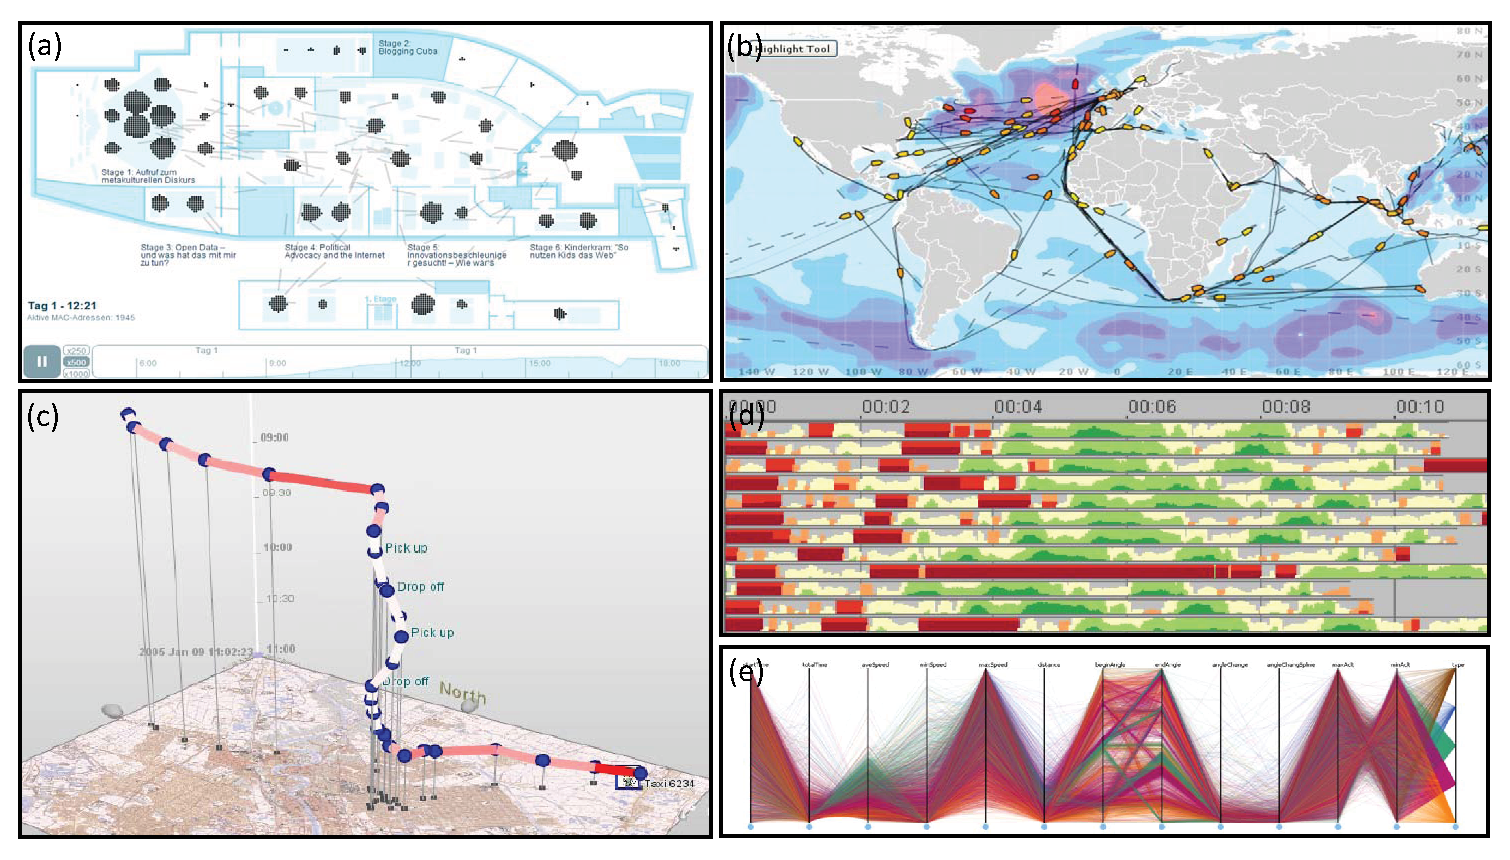
\includegraphics[width=0.85\linewidth]{images/direct.eps}
\caption{\label{fig:direct}轨迹数据的直接可视化。
%~(a)~人们参加会议时的位置动画~\citep{OpenDataCity2013}~。
%~(b)~船舶航行的路径可视化~\citep{LundbladEH2009}~。
%~(c)~个人移动轨迹的时空立方体可视化~\citep{EcclesKHW2007}~。
%~(d)~车辆行驶速度的时变可视化~\citep{TominskiSAA2012}~。
%~(d)~路口交通轨迹的属性可视化~\citep{GuoWYZY2011}~。
}
\end{figure*}

时空立方体技术~\citep{Hagerstrand1970}~可以精确的表现二维轨迹位置随时间的变化。
如图~\ref{fig:direct}(c)~,该技术使用~x~和~y~轴表示轨迹的二维位置,~z~轴表示时间。
这样,~z~方向的斜率就大致表示了移动速度。
在时空立方体中,人们可以比较容易的看到单条轨迹的高速运动和停止,
以及多条轨迹的相遇与分离。
~GeoTime~软件~\citep{KaplerW2004,EcclesKHW2007}~在时空立方体技术的基础上,进一步允许用户标注轨迹事件,
并可以将这些事件以文本的形式导出。
尽管时空立方体技术有众多的优点,但由于轨迹间严重的相互遮挡,它通常只能支持少数轨迹的可视分析。

时变可视化主要表现轨迹的属性或位置随时间的变化。它一般先轨迹简化成一个时变数据,
再使用基于时间轴方法展示时变信息。例如,~Tominski~等人~\citep{TominskiSAA2012}~的
工作中就使用了时间条带图,用以表示车辆行驶速度随时间的变化,如图~\ref{fig:direct}(d)~。
而~Wang~等人~\citep{WangY2014}~试验了多种轨迹属性的时变可视化,并使用了三维的时间折线图。
~Thudt~等人~\citep{ThudtBC2013}~进一步尝试了使用时间轴表示二维轨迹位置的变化。他们的主要方法是,
先对轨迹分段,然后将每段轨迹单独绘制在一个圆形的小窗口中,最后将这些小窗口排列在时间轴上。

属性可视化关注轨迹在各属性上的分布,以及不同属性之间的关系。它一般先将轨迹简化成高维数据,
再使用高维数据可视化的方法进行分析,例如平行坐标(~Parallel Coordinates~\citep{Inselberg1985}~)。
如图~\ref{fig:direct}(e)~所示,~Guo~等人~\citep{GuoWYZY2011}~在研究路口交通轨迹时,
使用平行坐标绘制了每条轨迹的多种属性,包括起始时间、移动物体类别、平均速度、最大加速度等。
他们研究了这些属性之间的关系,并通过属性筛选寻找到了一些异常交通事件。
~Lundblad~等人~\citep{LundbladEH2009}~则使用平行坐标研究了船舶航行过程中气象条件的影响。

\section{聚集可视化}
\label{section:aggregration}

当轨迹数目较大时,直接可视化由于轨迹间严重的相互遮挡问题已经不适用。这时,人们可以考虑使用聚集可视化。
在这种方法中,轨迹数据先经过聚集计算得到一些聚集数据,然后这些聚集数据被显示给用户观察。
聚集可视化的优点包括:

\begin{itemize}
	\item 可以支持大量轨迹的可视分析。
	\item 可以直接回答许多涉及聚集特性的问题。
	\item 计算机分担了一些低层次的分析任务,人的分析压力减轻了。
\end{itemize}

同时,聚集可视化也有一些缺点:

\begin{itemize}
	\item 聚集计算需要保留一些重要信息,同时丢弃一些不重要的信息。然而,有时候用户并不清楚哪些信息是重要的,
尤其是在探索性较强、分析任务不明确的时候。
	\item 聚集数据有时不容易理解,例如,北京市交通流量最大的地区一天内的最小流量。
	\item 聚集可视化难以研究轨迹间的相互作用和相对运动~\citep{AndrienkoA2010a}~。
	\item 聚集计算需要额外的编程实现。
\end{itemize}

轨迹数据的聚集计算在思想上和数据挖掘中的空间数据立方体~\citep{HanSK1998}~很相关。
它们都是基于一个多维数据模型,在每个维度上对数据做统计。对于轨迹数据,这些维度包括
时间(记为~$T$)、空间(记为~$S$~)、轨迹的路径(记为~$R$~)以及每个轨迹记录点上的属性值(记为~$A$~)。
基于所选维度的不同,~Andrienko~等人~\citep{AndrienkoA2010a}~将聚集可视化方法分为:
时空和属性聚集(~$S \times T \times A$~)、出发点-目的地聚集(~$S \times S$~)和路径聚集(~$R$~)。
下面将一一介绍这三种方法。

\subsection{时空和属性聚集}
\label{subsection:aggregation_sta}

时空和属性聚集方法可以只作用于单个维度,例如空间聚集(~$S$~)、时间聚集(~$T$~)、属性聚集(~$A$~);
也可以作用于多个维度,例如时间属性聚集(~$T \times A$~)、空间属性聚集(~$S \times A$~)、
时空聚集(~$S \times T$~)和时空属性聚集(~$S \times T \times A$~)。
这些方法的主要区别在于是否包含空间维度的聚集。因此本小节将先介绍时间和属性聚集,再介绍基于空间的聚集。

\subsubsection{时间和属性聚集}

时间聚集主要关注轨迹数目随时间的变化,这在许多系统中都属于基本功能。
如图~\ref{fig:direct}(a)~所示,~OpenDataCity~\citep{OpenDataCity2013}~制作的位置动画界面
下方的时间轴内嵌一个蓝色的直方图,表示参会者数量随着时间的变化。
用户可以利用该直方图直接跳跃到他感兴趣的时间段。
~Guo~等人~\citep{GuoWYZY2011}~的路口交通轨迹分析系统中也有类似的时间轴。

属性聚集主要关注轨迹属性的分布以及属性之间的相互关系,一个例子是Willems等人~\citep{WillemsHVJM2010}~设计的船舶安全监控系统。
如图~\ref{fig:aggregation_sta}(a)~,界面左侧的直方图显示了船舶数据在单个属性上的分布,而中央的轨迹属性关联表
(Trajectory Contingency Table)则显示了一对属性的相互作用。

时间属性聚集研究时间和属性之间的关系,主要是属性分布随时间的变化。
Zhao~等人~\citep{ZhaoFH2008}~的活动圆环图(~Activity Ringmap~)可以显示
人们不同类型活动的强度随时间的变化。
~Liu~等人~\citep{LiuGLLQN2011}~则通过类似的设计
来表示出租车数量和速度随时间的变化。
~Guo~等人~\citep{GuoWYZY2011}~使用主题河技术(~ThemeRiver~\citep{HavreHWN2002}~)
表现一个路口不同类型的交通流量随时间的变化。他们还在主题河中嵌入了一些白色小图标,
用来表示移动方向。

不同于以上工作,~Landesberger~等人~\citep{LandesbergerBAAT2012}~关注的是个体属性随时间的转换。
以人的活动轨迹为例,他们关心的是,在某段时间内有多少人的状态属性从“工作”转变为了“下班”,
之后又有多少人的状态属性从“下班”转变为了“在家”?
如图~\ref{fig:aggregation_sta}(b)~,他们采用了一个类似于平行集合(~Parallel Sets~\citep{KosaraBH2006}~)的设计方式,
其中每根轴表示一个关键的时间点,而相邻轴之间的条带表示了状态变化。条带前后的颜色对应了前后的状态,而条带宽度则对应
发生此种状态变化的人数。

\begin{figure*}[!htb]
\centering
\includegraphics[width=0.85\linewidth]{images/aggregation_sta.eps}
\caption{\label{fig:aggregation_sta}轨迹数据的时空和属性聚集可视化。
%~(a)~船舶安全监控系统中的轨迹属性直方图、轨迹属性关联表和地图~\citep{WillemsHVJM2010}~。
%~(d)~一群人的活动状态属性随时间的转换~\citep{LandesbergerBAAT2012}~。
%~(c)~赛车比赛中,所有赛车经过~17~个蓝牙传感器的次数统计~\citep{AndrienkoASLH2012}~。
%~(d)~美国特拉华海岸的船舶轨迹热度图~\citep{DelawareVesselHeatMap}~。
%~(e)~荷兰附近海域的船舶轨迹密度图~\citep{WillemsWW2009}~。
%~(f)~一只老鼠在笼子内的不同位置出现的次数和时间分布~\citep{BakMJK2009}~。
%~(g)~英国手机通话次数统计,采用~Voronoi~多边形空间划分~\citep{AndrienkoAMMP2010}~。
%~(h)~荷兰附近海域某时刻船舶的类型、航行方向和移动比例分布~\citep{ScheepensWW2014}~。
%~(i)~意大利米兰城不同区域的平均车辆行驶速度随时间的变化~\citep{AndrienkoA2008b}~。
%~(j)~纽约市不同区域的出租车上下客次数统计~\citep{FerreiraPVFS2013}~。
%~(k)~人们在不同地区的活动强度随时间的变化~\citep{ZhaoFH2008}~。
}
\end{figure*}

\subsubsection{基于空间的聚集}

空间聚集主要关注轨迹的空间密度绘制。该方法通常需要先将空间划分为有限个互不重叠的区域。
此后,系统会分别统计每个空间单元内轨迹或位置点的密度,
最后再将密度用各种形式展示出来。颜色最为常用,如图~\ref{fig:aggregation_sta}(d)(e)(g)(i)(j)(k)。
此外,还可以使用圆圈的大小(图~\ref{fig:aggregation_sta}(f)(h))、
柱状图的高度(图~\ref{fig:aggregation_sta}(c))或者三维曲面的高度。

不同空间聚集方法的主要区别在于所使用的空间划分方法的不同。最简单的情况是,
原始数据中的空间位置仅限于一些有限的预定义的地点,例如蓝牙传感器或无线网络接入点,
这时就不需要进行空间划分。图~\ref{fig:aggregation_sta}(c)~中赛车数据的可视化~\citep{AndrienkoASLH2012}~就是这样一个例子。
整个赛车场安装有~17~个蓝牙传感器,可以记录经过的赛车。红色的柱状图表示赛车经过每个传感器的次数。
为了显示每个预定义地点的时间信息,~Bak~等人设计了生长圆环图(~Growth Ring Map~)。如图~\ref{fig:aggregation_sta}(f)~所示,
这里研究的是~RFID~传感器记录的小鼠行为数据,当小鼠经过传感器时就会产生一条记录。
图中每个圆形图案对应一个传感器,其大小表示小鼠经过的总次数,颜色表示经过的时间。

大多数时候,轨迹数据中的空间位置是任意的,这时必须先进行空间划分。空间划分的方式
包括:按照屏幕像素划分、按照均匀网格划分、按照行政区域划分和按照数据本身的密度进行多边形划分。
如果按照屏幕像素划分,那么每个像素就对应了一个区域。
空间热度图(~Heat Map~)是这种划分下的一种典型的可视化方法。
图~\ref{fig:aggregation_sta}(d)~是美国特拉华海岸的船舶轨迹的热度图~\citep{DelawareVesselHeatMap}~。
该方法简单直接,应用最为广泛。不过,它存在一些不足。如图所示,右下方的颜色过于均匀,缺少信息量;
而左上方的颜色又比较杂乱,表现出的热度很不连续,而这种不连续一般是采样不足所造成的假象。
~Willems~等人提出的密度图(~Density Map~)~\citep{WillemsWW2009}~在这两点上要优于热度图,
如图~\ref{fig:aggregation_sta}(e)~。密度图使用核函数(~kernel~)对原始的密度进行了平滑。
特别的,这里通过使用两种不同大小的核,可以得到一个在空间上平滑变化的密度场~$D_1$~
和一个显示轨迹细节的密度场~$D_2$~。前者映射成颜色,保证了颜色的连续性;
后者映射成高度,结合光照效果能显示出轨迹细节。
在后续的工作中,他们支持使用不同颜色显示多个密度场,
这样就可以在密度图中显示时间和属性信息~\citep{ScheepensWWW2011}~。
他们还增强了空间密度图的表达性和灵活性~\citep{ScheepensWWAAW2011}~。他们允许用户对轨迹进行筛选,自己编辑公式计算新的属性值,
并且自己定义空间密度图的计算和渲染流水线。此外,~Peters~等人~\citep{PetersK2010}~尝试
在空间密度图中添加更明显的方向信息,而~Demsar~等人~\citep{DemsarV2010}~则尝试将密度图应用于时空立方体,但效果都不理想。
~Willems~等人~\citep{WillemsWW2011}~通过用户实验研究了密度图在轨迹分析中的实际效果。
结果显示,密度图主要强于表现轨迹中的停止特征。而对于其他一些特征的表现,
密度图可能略微差于动画或者时空立方体技术。

当用户需要更高层次的密度时,可以采用均匀网格划分。例如,
~Andrienko~等人将意大利米兰城划分成均匀网格区域,并绘制了各区域的交通流方向分布
和时间分布~\citep{AndrienkoA2008b}~。图~\ref{fig:aggregation_sta}(i)~是他们设计的用来表示交通流时间分布的
马赛克图表(~Mosaic Diagram)。他们在米兰城的每个区域内镶嵌了一个矩形的马赛克图案。
该图案有7列和24行,分别对应一周的7天和一天的24小时,颜色表示该区域在相应时刻的平均车辆行驶速度。
进一步,他们对时间和空间进行了聚类分析~\citep{AndrienkoABSVB2010}~。他们可以将不同的区域按照时间特征进行聚类,
也可以将不同的时间段按照空间特征进行聚类。
~Pu~等人的工作~\citep{PuLQN2012}~参考了马赛克图表。他们使用环形图案来表示城市各区域
车辆密度或者平均行驶速度随时间的变化。

用户也可以选择按照行政区域划分。如图~\ref{fig:aggregation_sta}(j)~,
~Ferreira~等人~\citep{FerreiraPVFS2013}~绘制了纽约市不同行政区域的出租车上下客次数。
Zhao~等人~\citep{ZhaoFH2008}~在行政地图上嵌入环形图案,
用以表示人们在不同区域的活动强度随一天24小时的变化,
如图~\ref{fig:aggregation_sta}(k)~所示。

以上的空间划分方法都没有考虑数据本身的空间分布,因此可能造成一些不理想的情况。例如,可能只有少数区域密度高,
而其他大部分区域密度极低。此外,数据自然形成的高密度区域更接近多边形的,而不是均匀网格
或者行政区域。为了解决以上问题,如图~\ref{fig:aggregation_sta}(g)~所示,
~Andirenko~等人~\citep{AndrienkoA2011}~发展了一种基于数据本身空间分布的多边形划分方法。
他们首先提取所有的轨迹记录点,或者只是其中的关键点。然后,他们对这些点进行密度聚类,并按照得到的点类位置
对空间做~Voronoi~划分。在后续的工作中~\citep{AndrienkoAMMP2010}~,他们将这种划分方法运用于分析手机通话数据
和~Flicker~上的照片数据。
~Scheepens~等人~\citep{ScheepensWW2014}~将某一时刻所有的船舶按照位置分成了许多簇。对于每一簇,
他们统计出了其船舶类型、航行方向和移动比例的分布,并用一个类似饼图的符号表现出来,如图~\ref{fig:aggregation_sta}(h)~。
他们的算法保证了这些绘制出来的符号不会相互遮挡。

\subsection{出发点-目的地聚集}
\label{subsection:aggregation_ss}

出发点-目的地聚集考虑的是物体在空间区域之间的移动,例如,从~A~区域到~B~区域平均每天有多少车辆经过?
这类聚集方法同样要求空间区域的数量是有限的,否则需要先进行空间划分。接着,这类方法会计算任何一对
区域之间的移动特征(例如流量)。
这样,轨迹数据实际上已经被转化成出发点-目的地数据(~Origin-Destination Data~,简称~OD~数据)。
~OD~数据描述的是物体在一对出发点、目的地之间的移动,如人口迁移数据。它和轨迹数据的区别是它不记录具体的移动路径。
因此,接下来任何~OD~数据的可视化方法都可以使用,包括:流向图(~Flow Map~)、~OD~矩阵(~OD Matrix~)和~OD~图(~OD Map~)。

\begin{figure*}[!htb]
\centering
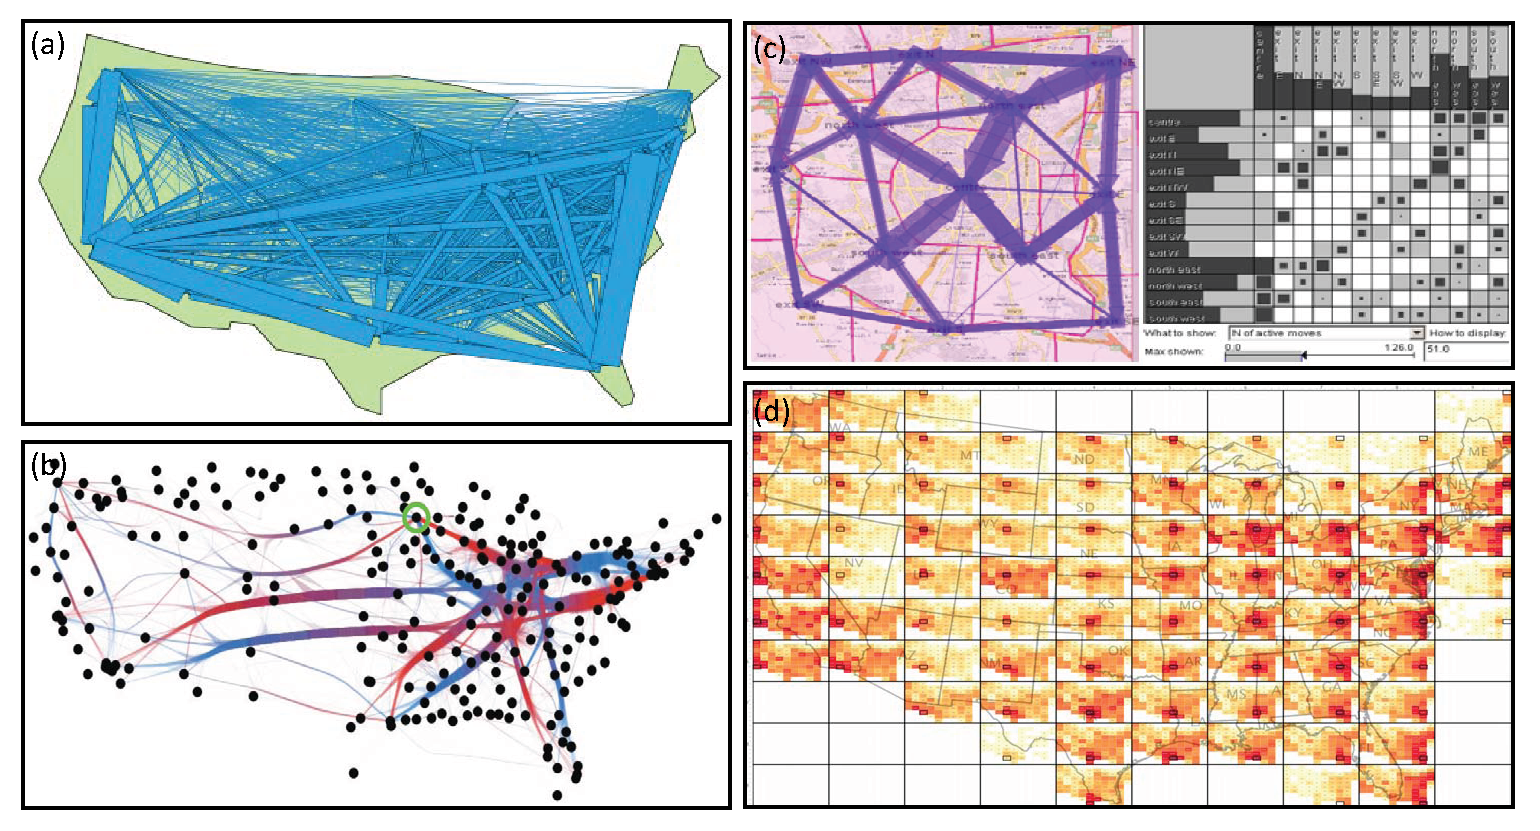
\includegraphics[width=0.85\linewidth]{images/aggregation_ss.eps}
\caption{\label{fig:aggregation_ss}轨迹数据的出发点-目的地聚集可视化。
%~(a)~美国人口迁移地图,直接用直线箭头绘制~\citep{Tobler2003}~。
%~(b)~美国国内航线地图,使用区分边方向的边捆绑技术绘制~\citep{SelassieHH2011}~。
%~(c)~意大利米兰城的交通流向图和~OD~矩阵~\citep{AndrienkoA2008b}~。
%~(d)~美国人口迁移地图,使用~OD~图绘制~\citep{WoodDS2010}~。
}
\end{figure*}

流向图最为直观,它在地图上的区域之间直接绘制有向边,并用边的宽度表示流量大小。~Tobler~\citep{Tobler1987}~很早就研究了流向图,
并绘制了美国的人口迁移地图,其中边的方向用箭头表示。流向图的主要问题是,当区域较多时,
边之间的相互遮挡成为一个严重的问题,如图~\ref{fig:aggregation_ss}(a)~。为了减少边遮挡,研究者们采取了各种各样的方法。
~Tobler~\citep{Tobler1987}~尝试了不同的箭头画法,并提出过滤掉一些流量小的边。
~Guo~\citep{Guo2009}~通过多层次的空间区域划分的方法来控制边的数量。
~Selassie~等人~\citep{SelassieHH2011}~采用了边捆绑(Edge Bundling)技术。
他们通过弯曲边,让相似的边相互靠近形成一束,以减少相互遮挡,如图~\ref{fig:aggregation_ss}(b)~。
目前的大部分的边捆绑技术都不支持边的宽度,因此无法用宽度表示流量大小。但是,如果用户选定一个中心区域,
只看和该区域相关的边,那么已经有技术可以利用边的宽度了~\citep{VerbeekKS2011}~。
流向图的一个变种是弧线图,其中不同的空间区域并非画在地图上,而是一字排开。区域之间使用弧线表示流。
~Nagel~等人~\citep{NagelMDMKK2014}~在研究单条公交线路上不同车站之间的流量时就使用了弧线图。

流通常有不同的属性,还会随时间变化。对于属性信息,最常用的方法是将属性值表示为箭头的颜色。然而,这种方法每次只能表现一个属性,
对于有多个属性的流,它无法同时表现所有属性。针对这个问题,~Guo~\citep{Guo2009}~对所有的流按照高维属性特性进行了聚类。
用箭头的颜色表示每一类流。对于时间信息,~Boyandin~等人~\citep{BoyandinBBL2011}~将流向图的三部分,
出发点、目的地和边,分别画在三个界面中。其中,出发点和目的地分在左右两张地图上。所有的边则按照时间对齐形成一张表,放在中间。
这样就更清晰的表示流的时间信息,并可以支持筛选排序等的分析任务。

~OD~矩阵的方法来自图的矩阵表示~\citep{HenryF2006}~。如图~\ref{fig:aggregation_ss}(c)~,~Andrienko~等人
~\citep{AndrienkoA2008b}~在研究意大利米兰的交通轨迹数据时,不仅使用了界面左侧的流向图,
还使用了右侧的~OD~矩阵。在矩阵中,每一行和每一列对应一个区域,而每个单元格对应一对区域间的流。
~OD~矩阵对于区域之间聚类性的显示比较清晰,但是在空间信息的表现上很不直观。

~Wood~等人~\citep{WoodDS2010}~提出的~OD~图利用嵌套的思想对~OD~矩阵空间信息不直观的问题进行了改进。
如图~\ref{fig:aggregation_ss}(d)~,他们在研究美国人口迁移数据时,将美国按照黑色的规则网格划分成一系列矩形区域。
这些得到的区域自然排列成了一个二维的矩阵。
接着,他们在每个单元格内再嵌套这样一个二维区域矩阵。这时,~A~区域单元格内嵌套的~B~区域单元格就对应~A~到~B~的流。
在后续的工作中,他们~\citep{WoodSD2011}~还将该方法用于研究英国伦敦的公共自行车数据。
~OD~图本来只适用于按照规则网格划分的空间区域,但~Slingsby~等人~\citep{SlingsbyKDW2012}~在研究爱尔兰不同行政区之间的人口迁移时,
手动将这些区域排列成矩阵。这样,他们就将~OD~图运用到了非规则网格划分的空间区域上。

\subsection{路径聚集}
\label{subsection:aggregation_r}

前面介绍的聚集方法都是建立在事先对空间、时间或者属性进行划分的基础上,而路径聚集与它们不同。
路径聚集研究轨迹在路径上的分布,然而这些路径事先是未知的。该方法先通过聚类算法得到经过不同路径的轨迹,
再将每类轨迹的路径显示出来。比较有代表性的轨迹数据聚类算法包括基于概率的聚类~\citep{GaffneyS1999}~、
基于分割的聚类(可以使用传统的~K-means~方法)、基于密度的聚类~\citep{EsterKSX1996}~、
基于子轨迹的聚类~\citep{LeeHW2007}~和基于流场的聚类~\citep{FerreiraKSS2013}~。
其中,基于分割和密度的聚类使用最为广泛。
它们都需要预先指定合适的轨迹相似性函数(或者距离函数)~\citep{PelekisAAKMT2012}~。
另外,当轨迹数据规模很大无法全都放在内存中时,大部分的聚类方法都无法运行。
针对这种情况,~Andrienko~\citep{AndrienkoARNPG2009}~等人提出了一些解决方案。

在实际问题中,面对复杂的轨迹数据,完全自动的聚类算法往往不能得到满意的结果。
因此,一些可视化研究人员发展了交互式聚类方法。
例如,~Rinzivillo~\citep{RinzivilloPNGAA2008}~等人
的渐进式(~Progressive~)的轨迹聚类系统,允许用户在聚类过程中依次采用多种相似性函数进行不同层次的聚类。
用户也可以选择一些轨迹或者一些已有的聚类,手动将其指定为一类或多类。图~\ref{fig:aggregation_r}(a)~展示了他们的聚类结果。
而~Schreck~等人的方法~\citep{SchreckBTK2008}~开发了一个基于~SOM~的半监督轨迹聚类系统。
用户可以在~SOM~聚类开始前指定神经元和参数,运行中动态观察新出现的模型
并评价当前聚类质量,完成后手动修改结果。图~\ref{fig:aggregation_r}(b)~展示了他们的系统界面。

\begin{figure*}[!htb]
\centering
\includegraphics[width=0.85\linewidth]{images/aggregation_r.eps}
\caption{\label{fig:aggregation_r}轨迹数据的路径聚集可视化。
%~(a)~渐进式轨迹聚类系统,允许用户不断调整相似性函数;得到不同类别的轨迹用不同的颜色
%一一绘制出来~\citep{RinzivilloPNGAA2008}~。
%~(b)~基于~SOM~的轨迹形状聚类系统,允许用户参与聚类过程~\citep{SchreckBTK2008}~。
%~(c)~一类轨迹的包围盒表示~\citep{BuliungK2004}~。
%~(d)~一类轨迹的流场表示~\citep{FerreiraKSS2013}~。
%~(e)~一类轨迹的系列箭头表示~\citep{AndrienkoARNPG2009}~。
}
\end{figure*}

对于轨迹聚类结果,最直接展示方法是把相应的轨迹一一画出来,如图~\ref{fig:aggregation_r}(a)~所示。
然而,这时轨迹间的相互遮挡经常会很严重。因此,许多时候人们会绘制一类轨迹的聚集结果。
如图~\ref{fig:aggregation_r}(c)~所示,~Buliung~\citep{BuliungK2004}~等人为一类轨迹构建一个多边形包围盒,
也可以进一步显示轨迹中心的移动趋势。
~Andrienko~\citep{AndrienkoARNPG2009}~等人则使用出发点-目的地聚集的方法,将一类轨迹聚集为一系列的区域间移动,
如图~\ref{fig:aggregation_r}(e)~。如果聚类本身是基于某种模型,那么对每一类轨迹可以显示对应的模型。
如图~\ref{fig:aggregation_r}(d)~所示,~Ferreira等人~\citep{FerreiraKSS2013}~的聚类算法将每一类轨迹拟合成一个流场。
因此,他们可以将相应的流场显示出来作为这一类轨迹路径的概括。

\section{特征可视化}
\label{section:extraction}

可视分析最终的目的是帮助人们发现和分析数据中的特征,从而获得知识。如果人们所关心的特征比较确定,并且能计算出来,
那么可以考虑特征可视化的方法。特征可视化先通过分析轨迹数据提取出特征,再将这些特征绘制出来。

特征可视化有一系列优点:

\begin{itemize}
	\item 可以支持大量轨迹的可视分析。
	\item 可以直接研究用户最关注的特征,在分析任务明确时通常能给出最相关的结果。
	\item 相对于依靠用户寻找特征,通过计算机自动搜索更加系统和高效。	
	\item 计算机分担了大量的分析任务,人的分析压力较小。
\end{itemize}

特征可视化的缺点有:

\begin{itemize}
	\item 特征计算丢失了与特征无关的大量信息,但是这些丢失的信息有时会和用户关注的特征有很强的相关性,甚至能够预测和解释这些特征。
	\item 特征计算要求用户很清楚自己的研究任务,并且能清楚的定义自己感兴趣的特征,因此对探索性较强的任务支持不好。
	\item 特征计算需要大量的编程实现。
\end{itemize}

特征可视化的方法大致可以分为事件可视化和模式可视化。事件可视化关注的是满足特定条件的部分轨迹及其相关的时间,
例如交通拥堵时间。模式可视化关注的是所有轨迹数据体现出的某种模式,例如道路通行状况随时间和路段的变化。下面将一一介绍。

\subsection{事件可视化}
\label{subsection:extraction_event}

根据~Andrienko~等人~\citep{AndrienkoAH2011}~的定义,满足一定条件的时间段称为事件。
如果事件同时有空间位置的话,就成为了空间事件。对于轨迹数据,事件通常对应一些轨迹片段,
并且同时有时间和空间信息,例如车辆慢行和老虎捕食。因此,轨迹事件都是空间事件。

在事件可视化的方法中,用户先提取事件,再对事件进行显示和分析。
事件提取可以基于简单的轨迹属性筛选~\citep{AndrienkoAHRW2013}~,例如“速度低于~10~米每秒的车辆轨迹”;
也可以通过复杂一些的查询语句来完成~\citep{SakrABAGH2011}~,例如“飞机在降落过程中突然向上飞行”。
有时候,事件提取也会需要用到专门的算法,例如相遇事件~\citep{BakMHYS2012}~
和低密度事件~\citep{DoraiswamyFDFS2014}~的提取。

\begin{figure*}[!htb]
\centering
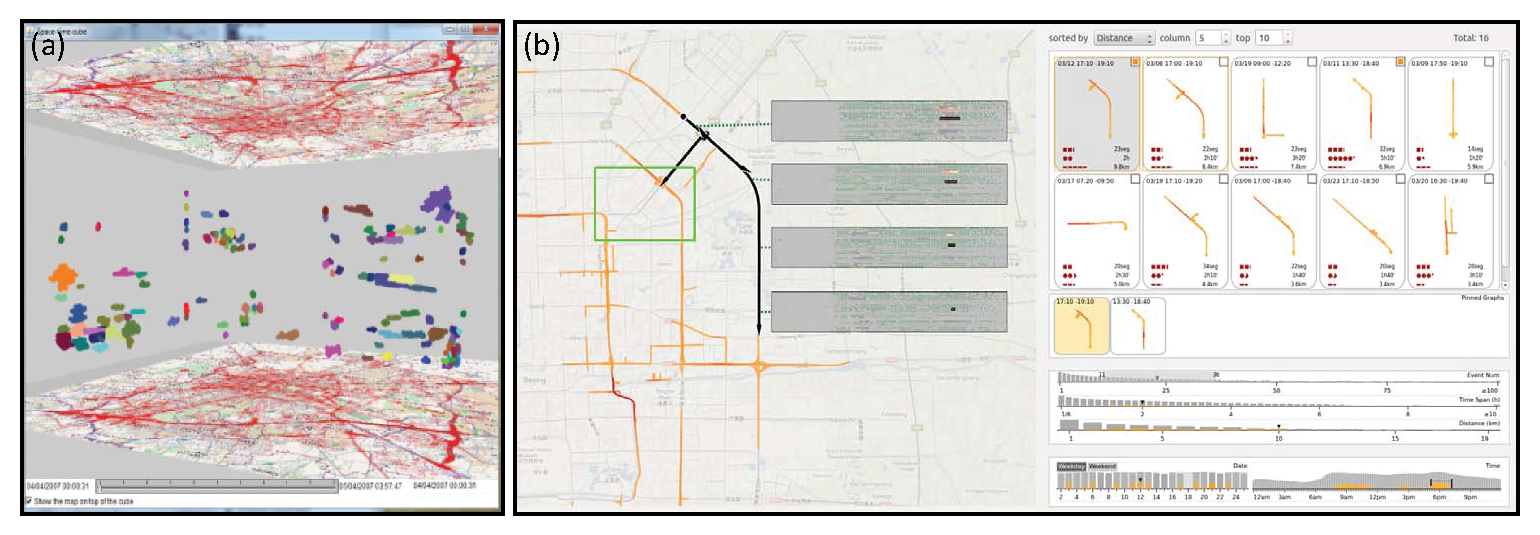
\includegraphics[width=0.85\linewidth]{images/extraction_event.eps}
\caption{\label{fig:extraction_event}轨迹数据的事件可视化。
%~(a)~车辆慢行事件的时空分布~\citep{AndrienkoAHRW2013}~。
%~(b)~交通拥堵事件在时间、空间、大小和拓扑结构上的分布,以及拥堵沿着路网的传播关系~\citep{WangLYZW2013}~。
}
\end{figure*}

事件提取将轨迹数据转化成了空间事件数据,接下来需要分析这些事件。
~Andrienko~等人~\citep{AndrienkoAWO2008}~在车辆的相遇事件分析中,
使用地图和时间条带图分别展示了事件的空间和时间分布。
此后,他们在研究车辆的慢行事件时~\citep{AndrienkoAHRW2013}~,
先根据空间、时间和行驶方向对事件进行了聚类,
然后对每一类事件使用不同的颜色,显示在时空立方体中,如图~\ref{fig:extraction_event}(a)~。
~Doraiswamy~等人~\citep{DoraiswamyFDFS2014}~在提取了出租车上下客次数异常低的事件之后,
很据相似性对这些事件进行了归类整理。然后,他们设计了一系列散点图,以支持用户对这些事件的探索。
~Wang~等人~\citep{WangLYZW2013}~在城市交通拥堵分析中,根据拥堵的传播关系,将不同路段上的拥堵事件
组织成了拥堵传播图。如图~\ref{fig:extraction_event}(b)~,用户可以查看单个传播图的细节,也可以
查看所有传播图的空间密度、时间分布、传播长度分布、传播时间分布以及拓扑聚类,
并据此进行筛选和排序。

Andrienko~等人~\citep{AndrienkoAHRW2013}~轨迹数据事件可视化的分析流程总结为
四个步骤:事件提取、地点提取、数据聚集、交互分析。
以车辆轨迹数据为例,假定分析目标是研究城市的交通拥堵。首先,用户可以从轨迹数据出发,
通过速度属性提取车辆的慢行事件。之后,用户通过对这些事件按照空间位置和行驶方向聚类,
可以得到城市中经常拥堵的地点。依据这些事件和地点,用户可以计算出各种聚集数据,
例如空间密度、时间分布、属性分布。最终,这些聚集数据将显示给用户,
以支持用户的交互式分析。

\subsection{模式可视化}
\label{subsection:extraction_behavior}

模式可视化研究的是所有数据中,某个特征随时空和属性的变化模式。按照~Dodge~等人~\citep{DodgeWL2008}~基于移动特征的分类,
模式可视化既可以关注一般特征也可以关注行为特征。一般特征适用于几乎所有的轨迹数据,而行为特征只在特定的应用中有意义。
对于一般特征,目前研究较多的是多个轨迹之间的相互关系,例如移动物体的相对位置。研究者会为这些量设计可视化的表达方式。
对于行为特征,如果研究目标不是很明确,这时研究者会从轨迹中挖掘一些低层次的语义信息,例如每段轨迹对应移动者的何种活动。
原始数据和这些语义信息会被一起呈现给分析人员,以支持一些简单的交互式探索。如果研究目标很明确,
那么研究者会直接计算出特征并显示出来,例如出租车司机寻找乘客的策略。本小节将以上三种情况简称为:
一般特征模式可视化、探索式的行为特征模式可视化和目标明确的行为特征模式可视化。下面一一介绍。

\begin{figure*}[!htb]
\centering
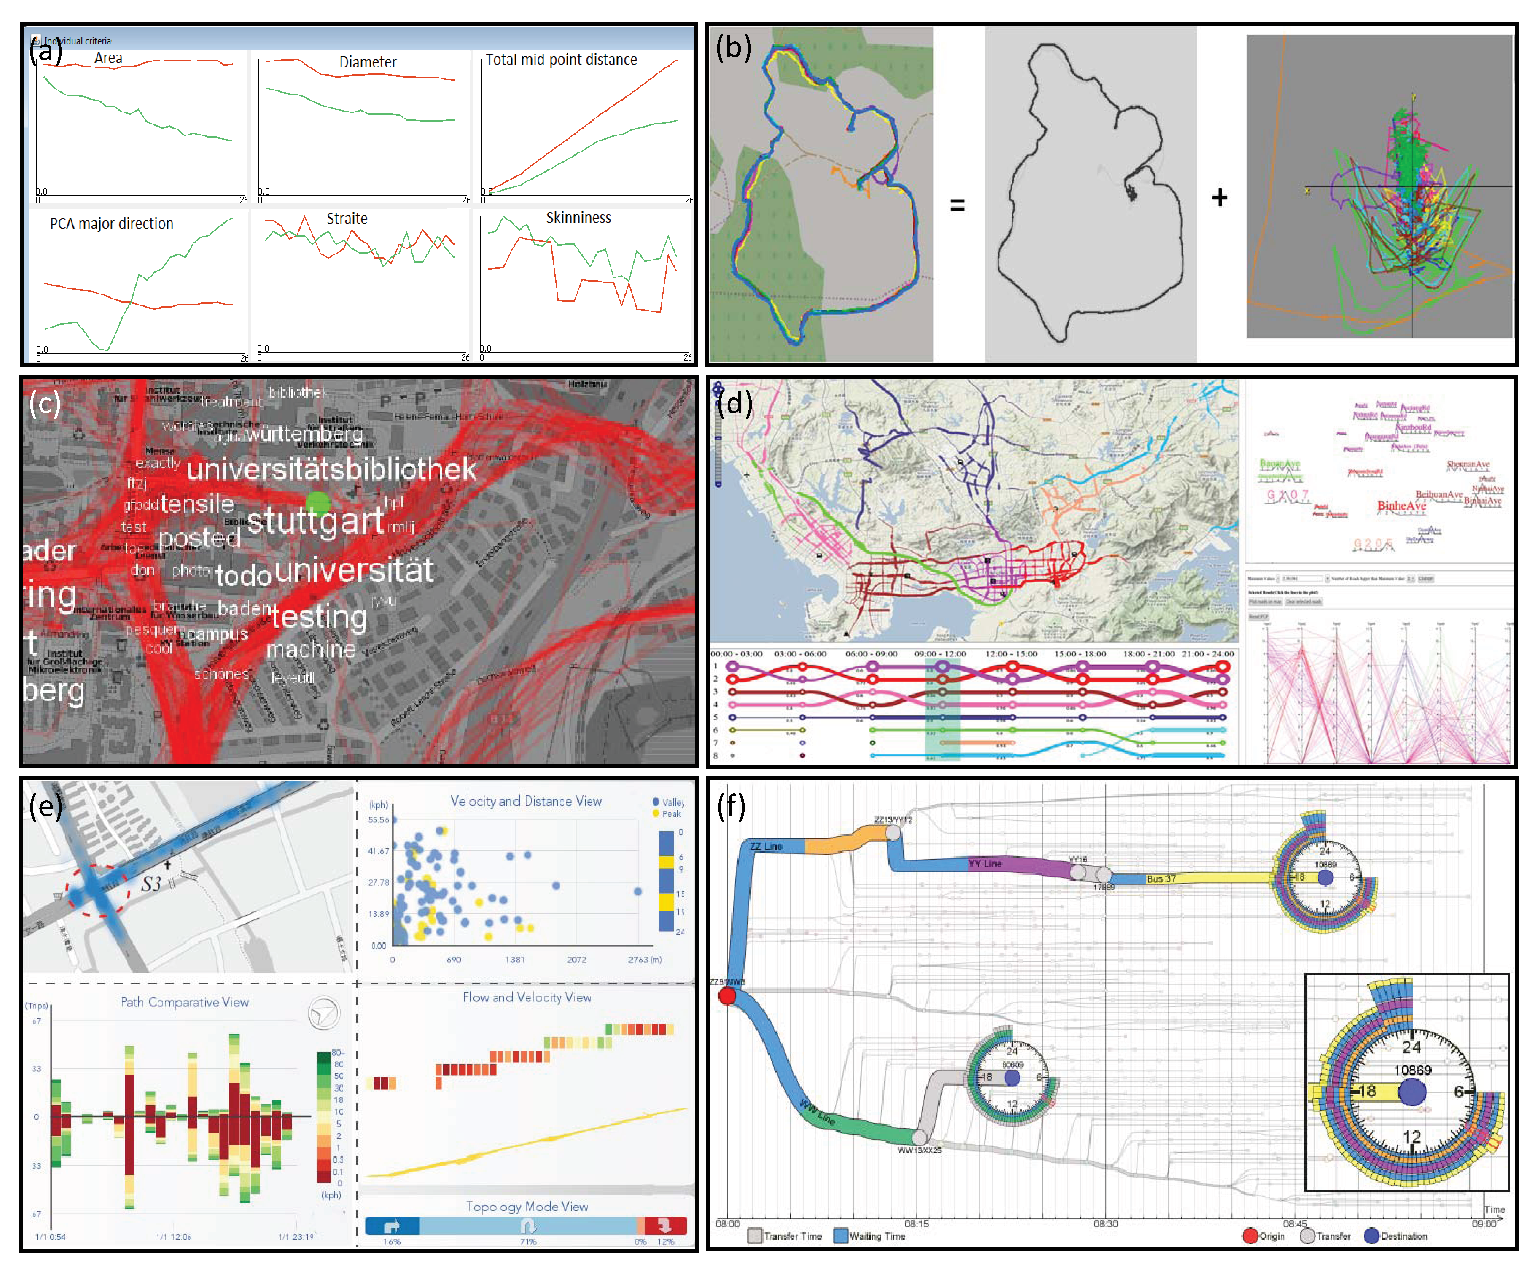
\includegraphics[width=0.85\linewidth]{images/extraction_pattern.eps}
\caption{\label{fig:extraction_pattern}模式可视化。
%~(a)~一群移动物体的群体属性随时间的变化,包括包围盒面积、直径等~\citep{LandesbergerBSF2012}~。
%~(b)~一群人的移动轨迹可以分解为群体中心的轨迹加上每个个体相对于群体中心的位置变化~\citep{AndrienkoABDH2013}~。
%~(c)~通过~Twitter~文本数据来标注轨迹的目的地语义~\citep{KrugerLTBE2012}~。
%~(d)~通过文本挖掘中的~LDA~方法得到出租车轨迹形成的“话题”,并分析了这些“话题”的
%空间分布、时间变化和内部含义~\citep{ChuSZWYZ2014}~。
%~(e)~城市中单条道路流量、速度等状况的可视化~\citep{WangCWZHG2014}~。
%~(f)~乘客从一个公交或地铁站点出发,到达其他站点的时间花费模式可视化~\citep{ZengFAEQ2014}~。
}
\end{figure*}

\subsubsection{一般特征模式可视化}

当研究的特征是标量时,通常可以使用简单的可视分析方法。
例如,~Crnovrsanin~等人~\citep{CrnovrsaninMCM2009}~使用一个简单的时间折线图
表现了不同动物到临近水源的距离随时间的变化。
而在图~\ref{fig:extraction_pattern}(a)~中,~Landesberger~等人~\citep{LandesbergerBSF2012}~
同样使用时间这些图展示了一些群体移动特征随时间的变化。

当研究的特征是位置时,可以采用空间变换的方法。如图~\ref{fig:extraction_pattern}(b)~所示,
~Andrienko~等人~\citep{AndrienkoABDH2013}~将一群共同移动的人的轨迹分解为群体中心
的移动加上个体相对于群体中心的位置变化。后者显示了个体间的相互关系,以及他们在群体中的角色。
~Crnovrsanin~等人~\citep{CrnovrsaninMCM2009}~通过~PCA~变换,将原本在自然空间中密集分布的轨迹
分散开来,从而展示出更多细节。

相比于空间变换方法,~Chavoshi~等人~\citep{ChavoshiBNTW2012}~采取了更为直接的抽象编码方法来分析位置特征。
他们在研究人四肢的运动轨迹时,对时间信息以及四肢间相对距离的增减进行了编码。最终,他们采用一系列的嵌套方格恶的形式,
来表现不同运动模型出现的频次。

\subsubsection{探索式的行为特征模式可视化}

在行为特征的可视分析中,如果研究目标不是很明确,研究者会从轨迹中挖掘一些低层次的语义信息,以辅助探索。
~Parent~等人总结了~\citep{ParentSRAAB2013}~处理轨迹数据中语义信息的方法,并将其分为两大类:语义充实(~Semantic Enrichment~)、
行为知识提取(~Behavior Knowledge Extraction~)。其中,语义充实指的是为轨迹数据中的整条轨迹或者每个轨迹点添加表示语义的属性,
例如每个点可以添加“工作”、“在家”等活动状态。行为知识提取则是指对轨迹数据使用数据挖掘方法,
如分类、聚类、共同序列发现或者相互关系分析。

Spretke~等人~\citep{SpretkeBJKMD2011}~在分析鸟类迁徙的轨迹数据时,
根据几何特性对轨迹进行了切分,并对子轨迹再聚类。接着,他们允许用户根据自己的经验,将每一类子轨迹标注成一类行为。
~Krüger~等人~\citep{KrugerLTBE2012}~在分析了自行车轨迹终时,搜索了终点附近的~Twitter~数据,并提取出关键词
标注在了地图上,如图~\ref{fig:extraction_pattern}(c)~。由此,用户可以根据关键词大致猜测出这些轨迹的语义。
在后面的一个工作中~\citep{KruegerTE2014}~,他们又尝试根据终点附近的兴趣点(POI)来研究轨迹的语义。
~Andrienko~等人~\citep{AndrienkoAF2013}~将人在不同位置之间的移动轨迹转换为在不同语义位置之间的移动,
并用流向图展示出来。

Ding~等人~\citep{ChuSZWYZ2014}~借用了文本分析中的~LDA~方法,提取了出租车数据的“话题”。
其中,每个话题以一定的概率包含某些道路,而每条出租车轨迹则以一定的概率属于某些话题。
接着,他们通过地图、时序图、火花谱线云(~Spark Cloud~)等方式显示了不同话题的时空分布
,如图~\ref{fig:extraction_pattern}(d)。

\subsubsection{目标明确的行为特征模式可视化}

在行为特征的可视分析中,如果研究目标很明确,那么就可以直接计算出特征并显示出来。
使用这种方法的研究工作一般都和具体的应用问题结合很紧密,其具体可视化方案也因应用的不同而不同。下面举一些例子来说明。

在城市交通状况分析方面,Wang~等人~\citep{WangCWZHG2014}~关注单条道路的状态。
当用户选定一条道路时,系统会自动提取经过这条道路的出租车轨迹,并计算出其速度、流量、密度的时空分布,
以及进出路段的拓扑类型分布。在此基础上,他们设计了
地图、道路双向交通流比较、速度距离、速度流量、拓扑分布等多个视图,
从多个角度支持用户的分析,如图~\ref{fig:extraction_pattern}(e)~。
~Wang~等人~\citep{WangYLYQY2014}~的研究使用了新型的智能交通基站数据。
他们除了展示基站处交通的流量、速度变化模式,还允许用户研究一个基站拥堵时周围道路流量的变化,
由此分析拥堵的原因或者影响。

在城市交通可达性分析问题,Zeng~等人~\citep{ZengFAEQ2014}~计算了
乘客从一个公交或地铁站点出发,到达其他站点的时间花费。他们设计了多种
可视化形式,包括一个可达性地图,以及图~\ref{fig:extraction_pattern}(f)~中的旅程图。在该图中,横轴表示时间,
左边的红点表示从起点出发,而右侧的分支表示到达其他各个站点。这里有两个终点被选中,然后系统显示了在不同时间出发抵达这两个终点
所需时间的变化,以及在当前时刻出发的预计的旅程中不同段的时间花费。~Wu~等人~\citep{WuZQCGN2014}~采取了另一种研究方法。
他们计算了不同时刻的可达性边界,并设计了~BoundarySeer~系统用于分析了该边界随时空的变化情况。

除此之外,Liu~等人~\citep{LiuGLLQN2011}~研究了出租车路径选择的多样性,
~Zeng~等人~\citep{ZengFAQ2013}~研究了乘客在地铁站内的换乘模式,
而~Gao~等人~\citep{GaoXLLLQ2012}~研究了出租车司机的载客策略。

\section{用户交互}
\label{section:interaction}

对于轨迹数据,用户的交互主要包括在可视化界面中的进行数据排序、筛选和参数调节,以及对分析算法进行的模型选择和参数调节。
其中,数据排序、模型选择和参数调节一般通过标准的控件完成,而数据筛选,特别是涉及空间的数据筛选,
则需要交互设计。轨迹数据的空间筛选按照任务可以分为两类:根据路径的筛选和根据位置的筛选。
前者筛选给定时间段内,符合某种路径条件的轨迹;后者筛选某一时刻处于某位置的移动物体。

根据路径的筛选需要用户指定路径条件。~Chang~等人~\citep{ChangHN2012}~根据用户刷选的区域形状,
选择最相似的轨迹。~Guo~等人~\citep{GuoWYZY2011}~研究了三种主要的路径条件:
经过的位置、起始和终止位置、几何形状。如图~\ref{fig:interaction}(a)~所示,以路口交通轨迹数据为例,
如果需要选择经过某位置的轨迹,则可以在地图上圈选出该位置;如果需要选择从特定方向进入和离开路口的轨迹,
可以通过环形滑动条指定相应的方向;如果需要选择具有特定几何形状的轨迹,可以在地图上画出相应的形状,
并让系统自动匹配形状相似的轨迹。~Hurter~等人~\citep{HurterTC2009}~进一步研究了使用经过位置条件的筛选,
并提出了“刷选-选取-放下”的筛选流程。如图~\ref{fig:interaction}(b)~所示,他们首先通过涂刷的方式定义空间区域,
接着可以将选中的轨迹直接拖拽出来,同时产生一副新的可视化图片。在新的图片中,用户可以重复该流程,做进一步的筛选。
~Ferreira~等人~\citep{FerreiraPVFS2013}~允许用户使用
圈选加箭头的方式表示指定起始和终止位置,如图~\ref{fig:interaction}(c)~。~Krüger~等人~\citep{KruegerTWBE2013}~
则允许用户通过环形镜头来指定轨迹的起始终止位置,以及途经位置,如图~\ref{fig:interaction}(d)~。

根据位置的筛选需要用户先选中一个时刻,再选择一个位置区域。
~Bouvier~等人~\citep{BouvierO2008}~允许用户通过一个时间轴来选择时间,再在地图上选择区域。
用户可以改变时间,查看刚刚选中的移动物体在其他时间的位置分布。
在~OpenDataCity~\citep{OpenDataCity2013}~制作的动画中,则提供了更加灵活的交互。
如图~\ref{fig:interaction}(e)~所示,系统默认播放会场动画。
但是,当用户点击地图时,动画立即暂停,当前时刻自动被选中。于是,用户可以不放开鼠标直接拖出一个矩形的空间区域,
作为空间选择。选中的参会人员对应的点变为红色。

\begin{figure*}[!htb]
\centering
\includegraphics[width=0.85\linewidth]{images/interaction.eps}
\caption{\label{fig:interaction}轨迹数据的空间筛选交互方法。
%~(a)~针对路口交通轨迹数据的三种空间筛选方法,从左到右依次根据经过的位置、进入和离开路口的方向以及轨迹
%的形状指定筛选~\citep{GuoWYZY2011}~。~(b)~流畅的“刷选-选取-放下”筛选流程,应用于飞机轨迹~\citep{HurterTC2009}~。
%~(c)~通过选择经过区域或者一对起止区域,选择出租车轨迹~\citep{FerreiraPVFS2013}~。
%~(d)~通过多个环形镜头,选择经过特定起止区域和途经区域的人的轨迹~\citep{KruegerTWBE2013}~。
%~(e)~选择在某时刻恰好在会场某位置的参会人员~\citep{OpenDataCity2013}~。
}
\end{figure*}

\section{问题与挑战}
\label{section:challenge}

尽管研究者们已经进行了许多研究工作,并解决了不少问题。但是随着轨迹数据的大量产生和社会的高速发展,新的问题一直在不断被提出。
本节将列举一些重要的和有挑战性的问题。

首先,大量的轨迹数据需要有合适的存储和查询方式。
尽管目前已经有专门的轨迹数据库~\citep{GuetingBADHS2004},然而对于大数据,一条简单的查询
也可能需要数小时才能返回结果,这导致交互式的可视分析几乎无法进行。
可视分析研究者已经在大数据方面做了一些探索性的工作。例如,
~Lins~等人~\citep{LinsTKS2013}~针对空间点数据设计了类似数据立方体的聚集机制,
并构建了特殊的数据结构来存储这些聚集数据。这样,他们的系统可以利用有限的内存,实时返回~GB~量级数据的聚集属性查询结果。
~Fisher~等人~\citep{FisherPDm2012}~则通过一些用户研究说明,大数据的查询结果可以通过一系列小样本的查询结果来逼近。
在他们的系统中,每次小样本查询都返回查询结果和误差估计。系统会自动的不断增大样本容量,更新查询结果和误差估计。
当用户认为结果已经足以支持决定时,就可以停止查询。这样原本需要半天的查询可能在十分钟内就完成了。

使用可视分析技术帮助进行轨迹数据的预处理也是一个可能的研究问题。在大部分真正的数据分析中,最为耗时的步骤可能都是数据预处理。
轨迹数据也是如此。以轨迹数据的清理为例,原始的轨迹数据中总是存在大量的错误和信息缺失。对于这些错误和缺失的处理,
人们通常没有一个固定算法,因为不同的数据中会有不同的错误。很多预处理中的决定都依赖于分析人员的经验和对问题的理解。
然而,对于大量的轨迹数据,让人一条轨迹一条轨迹的清理显然是不现实的。因此,计算机的自动高效处理不可或缺。
从直觉上来看,可视分析结合了人的智慧和计算机的高效,应该很适合解决预处理的问题。
然而事实上,目前这方面的工作还很少~\citep{LiaoYC2010,LuCLNYQ2014}。

可视分析研究需要与应用领域更好的结合。可视分析系统是为了解决实际问题的,因此需要集成特定应用领域的自动分析方法。
此外,由于可视分析系统的用户往往是应用领域的分析人员,因此交互的设计也需要符合他们的习惯。
为了做到这些,可视分析研究人员需要对应用领域的现有研究问题和方法有较深入的了解,并与应用领域的专家保持充分的沟通和长期的合作。
最终,只有应用领域的专家才能够评价可视分析系统是否真的能帮助他们研究问题。然而,与应用领域的专家合作往往存在许多交流问题,
并且会使得系统的设计周期很长。此外,应用领域的专家需要的功能也许在可视分析研究者看来并没有研究价值,
而可视分析研究人员可能也没有足够的精力去实现和维护一个完整、正确和可用的系统提供给应用领域专家。
因此,将可视分析研究和应用领域更好的结合是一个很困难的问题。

最后,自动分析和交互式的探索需要更好的结合。这种结合是可视分析技术最重要的特点。然而,在目前的系统中,
分析基本上仅限于描述性的和探索性的分析,例如查看数据分布、寻找异常行为。尽管这两种分析很重要,
它们却并不足以解决实际问题。实际问题需要确定性的答案,例如明天交通会拥堵吗?什么导致了交通拥堵?
采取何种措施才能缓解交通拥堵?回答这些问题需要推断性的、预测性的和因果性的分析,甚至需要建立能精确模拟现实情况的机械性模型。
因为问题本身的复杂性,这些分析并不能完全自动完成,其中的参数选择和模型设计和模型评价等问题需要大量的人工干预。
但是,这些分析涉及的用户交互可能与描述性和探索性的分析是不同的。可视分析技术需要更多的考虑这些类型的分析任务。

\section{结论}
\label{section:conclusion}

本文概述了轨迹数据可视分析的主要方法以及交互设计。未来越来越多的轨迹数据将被采集和记录,
而轨迹数据可视分析的需求也将持续增长。目前该领域仍然存在许多重要的问题和挑战,需要继续研究。

\bibliographystyle{abbrvnat}
%\setcitestyle{aysep={,},yysep={;}}
\bibliography{trajsurvey}

\end{CJK*}
\end{document}

